\section{Overview of mmprof}

\MP{} aims to identify important factors of memory allocators, including the performance, the memory and the scalability issues. \MP{} reports some counter information, such as runtime per allocation/deallocation, memory overhead, or lock contention issues. It could further present some internal reasons of causing the issues, by intercepting synchronizations, system calls, and employing hardware performance counters. For instance, the DieHarder allocator is slow in its deallocation, mainly due to the use of a central lock (therefore causing the high contention), the large number of cache misses, and other reasons (as described in Section~\ref{}). Overall,  \MP{} not only uncovers potential issues, but also present some specific reasons of issues that could help programmers to solve these issues. \MP{} is designed as a drop-in library that can be simply linked to applications (and allocators) with the preloading mechanism, which does not require the change or the re-compilation of applications and allocators (mostly). %Although \MP{} may employ the binary instrumentation to perform a more detailed profiling, such as identifying the instructions within each allocation or deallocation, the binary instrumentation may impose prohibitive performance overhead. With a high overhead, the profiling results may be significantly skewed, such as the waiting time of each lock acquisition inside the allocation. Instead, \MP{} employs the PMU hardware, RDTSC timestamp hardware, and simple counters together to perform the profiling. 

Sine \MP{} aims to discover the issue inside allocations and deallocations, it intercepts the interfaces between applications with the memory allocator, such as invocations of memory-related APIs, such as \texttt{malloc}, \texttt{free}, \texttt{calloc}. Also, it also intercepts the interactions between the allocator with other components of the system, such as the OS (e.g., memory related system calls), and the pthreads library (e.g., synchronizations). By intercepting system calls, it could reveal whether an allocator causes significant kernel contention. From synchronizations, it could tell the scalability design of an allocator. As shown in Figure~\ref{fig:basicidea}, \MP{} also employs hardware performance counters to collect hardware information inside and outside the allocation/deallocation, such as the instructions, cache misses, or TLB misses of each allocation and deallocation. All the information reported by \MP{} helps programmer to identify the particular design issues inside the allocator.  
 
\begin{figure}[!ht]
\centering
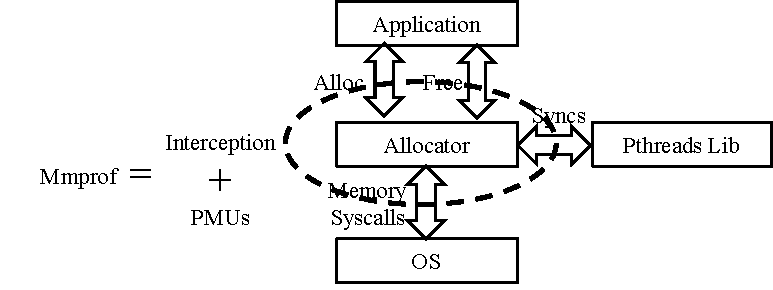
\includegraphics[width=5.5in]{figures/basicidea}
\caption{Basic Idea of mmprof\label{fig:basicidea}}
\end{figure}

Overall, \MP{} focuses on the allocator itself and its potential impact on applications (called as ``application friendliness''). These factors, when combined together, explain the performance difference of different allocators on different applications. \MP{} can assist allocator developers to identify the potential design issue, without writing a custom profiler. It could also help a user to choose an appropriate allocator for specific applications. In the remainder of this section, we describe the basic idea of its profiling. 

\subsection{Basic Idea}
\MP{} profiles the performance overhead, the memory overhead, and the scalability issues of allocators. Additionally, it also identifies whether an allocator is performance-friendly to a specific application, called as ''\textit{application friendliness}''.  


\begin{table}[h]
  \centering
  \footnotesize
 % \setlength{\tabcolsep}{1.0em}
\begin{tabular}{l | l | l}
\hline
Category & Collected Data & Collection Methods \\ \hline
\multirow{2}{*}{Performance Overhead} & {Alloc/Free runtime} & Simple Counter, RDTSC Timestamp\\ \cline{2-3}
& {Cache misses, page faults, TLB misses, instructions} & Performance Monitoring Units (PMU) \\ \hline
\multirow{2}{*}{Memory Overhead} & Internal fragmentation & Simple counter\\ \cline{2-3}
& {External fragmentation, memory blowup} & Simple counter \\ \hline
\multirow{2}{*}{Scalability} & Lock's acquisition, contention rate, runtime & Simple counter, RDTSC timestamp\\ \cline{2-3}
& {Number and runtime of related system calls} & Simple counter, RDTSC timestamp \\ \hline
{Application Friendliness} & Cache/page utilization rate, cache conflicts & Simple counter, PMU \\ \hline
  \end{tabular}
  \centering
  \caption{Profiling data and methods of \MP{}.\label{table:alldata}}
\end{table}


\subsubsection{Performance Overhead}

For the performance overhead, \MP{} collects the  data of each allocation and deallocation, instead of the summarized values over the whole execution. Each allocation/deallocation data helps identify potential issues inside, if the data is counterintuitive. \MP{} collects the following performance data. 

First, \MP{} collects the runtime of each allocation and deallocation with the RDTSC instruction, as further described in Section~\ref{}.  \MP{} utilizes the RDTSC instruction to collect the timestamp before and after each operation, and uses the difference of timestamps as the runtime of a specific operation. In its implementation, \MP{} further differentiates the runtime for different types of allocations, such as new/re-used allocation of small and large objects, as further described in Section~\ref{sec:performanceimplement}. 

Second, \MP{} also collects hardware events for each allocation and deallocation, such as cache misses, page faults, TLB misses, and instructions. These events enable the capability to discover a specific design issue without explicit instrumentation. For instance, a large number of instructions possibly indicates a questionable design of the allocator. 

%For instance, the \texttt{DieHarder} allocator is observed to have a very high number (\todo{up to X $\times$}) of cache misses upon each deallocation.  By examining the code, we found out a serious implementation issue of the DieHarder allocator, which traverses all mini-heaps to identify the placement of each object, causing excessive cache misses upon each deallocation.  

%Based on our understanding, the hardware events, such as retired instructions, cache misses or TLB misses, will help reveal some implementation issues of an allocator. For instance, \MP{} detects that the DieHarder allocator has an excessive number of cache misses and TLB misses upon each deallocation, around 5 times of each deallocation, which is significantly larger than that of other allocators. By examining the code, we found out a serious implementation issue of the DieHarder allocator, which traverses all mini-heaps to identify the placement of each object. Obviously, this implementation is extremely slow, considering that every deallocation has to perform such expensive lookup. By fixing such issues, the DieHarder's performance improves around \todo{20\%}.     


\begin{comment}
Can we integrate the cache misses or page faults for each allocation and deallocation, so that we could identify the issue of DieHarder that invokes many unnecessary cache misses?

If we could correlate cache misses to each thread, then we could do this. 

If allocation and deallocation takes too much time, it could be caused by multiple reasons:

(1) First, it just takes a lot of instructions (could we find out the lapsed instructions for each thread?)
(2) It may be caused by not good algorithm? 
(3) It can be caused by lock contention?
(4) It can be caused by system call related contention?
\end{comment} 

\subsubsection{Memory Overhead}

The memory overhead of an allocator comes from multiple aspects, including metadata overhead, internal fragmentation, external fragmentation, memory blowup, or explicit objects skipping. The metadata is used to track the available objects of each heap and the size information of each object. Based on our understanding, the metadata information is relatively small comparing to other memory overhead, which is omitted by \MP{}. 

Internal fragmentation is caused by the use of of size classes. Allocators manage heap objects using size classes in order to enable memory re-utilization. The difference between the requested size and the size of the corresponding class is internal fragmentation, which cannot be utilized to satisfy other requests. 

External fragmentation occurs, when the total amount of the available memory is sufficient to satisfy a request but fail to do so due to non-contiguous memory. External fragmentation is also related to the use of size classes. Most performant allocators rarely or never perform objects coalescing and splitting, since it is extremely expensive to perform these operations. Further, it is impossible to change the size class for only few objects in BiBOP-style allocators, since BiBOP-style allocators typically use a single size for all objects in the whole bag. That is, objects cannot be changed to other size classes, until all objects in the whole bag are freed. This design may cause extensive external fragmentation overhead. 

Memory blowup is caused by the use of multiple heaps for the scalability purpose, where memory deallocations from one heap can not be utilized to satisfy the concurrent memory requests of another heap~\cite{Hoard}. In order to solve this issue, Li et. al. employ heuristics to adjust the synchronization frequency dynamically~\cite{DBLP:conf/iwmm/LiLD19}. Since modern allocators typically utilize per-thread heap or arena to reduce the contention overhead, the memory blowup will be a big source of memory consumption. 

Secure allocators typically skip some objects in order to improve the security or reliability of the heap~\cite{DieHarder, openbsd, Guarder}. For instance, if a buffer overflow lands on non-used objects, it will cause no harm to the applications. However, it is extremely difficult to differentiate explicit skipping and external fragmentation. 

For the memory overhead, \MP{} will report the memory overhead caused by internal fragmentation, memory blowup, and other overhead. 

%It is relatively easy to compute the alignment overhead, as far as the information of size classes is known, which \MP{} utilizes a pre-run program to obtain (as described in Section~\ref{sec:understandingallocators}). \MP{} tracks each memory allocation, and then computes the alignment overhead for each allocation request. \todo{Of course, upon the deallocation, the corresponding alignment overhead will be extracted from the current overhead. But how we could know the actual alignment overhead for each object? It seems that we should store the information of such objects, or we could recompute due to the last object. }

\todo{For the memory blowup overhead, \MP{} profiles two types of blowup overhead. One type is simply based on the size of freed objects. If the total size of freed objects is larger than the requested size, but an allocation is satisfied from never-allocated objects, which is consider to be a memory blowup. Another type is based on the total size of freed objects with the same size. } 

%However, it is extremely challenging to compute  the metadata overhead, since it is difficult to identify the location of the metadata, without knowing (or changing) the detailed design of an allocator. \MP{} proposes a novel way to get the metadata overhead, based on the equation~\ref{eq:memoryoverhead}. That is, the metadata overhead can be computed if the total memory overhead ($Total\_{OH}$), alignment overhead ($Align\_{OH}$), or memory blowup ($Blowup$) is known.   

\begin{comment}
\begin{equation}
%\vspace{-0.1in}
\label{eq:memoryoverhead}
Total\_{OH}=Metadata\_{OH}+Align\_{OH}+Blowup
\end{equation} 

That is, we could compute the metadata overhead if we could know the total overhead of the heap, given that $Blowup$ and $Align\_{OH}$ can be computed as described above. The total memory overhead is the difference between the total memory consumption of heap objects and the total requested size of heap objects. For the latter one,  \MP{} could increment the size of every allocation, and then decrement the corresponding size of each deallocation.  That is, the question attributes to the determination of the memory consumption of the heap. We noticed that the \texttt{/proc/PID/smaps} file actually contains the size of physical memory for each virtual memory region (in its \texttt{Referenced} field). That is, we could compute the total physical memory consumption by summing up all physical memory of virtual memory regions that are related to the heap. In order to identify all virtual memory regions belonging to the heap, \MP{} intercepts all memory related system calls, and only includes those ones invoked during allocations and deallocations. 

 


%How we could know the total memory consumption? As described in Section~\ref{}, \MP{} intercepts all memory allocations and deallocations. Also,  all memory-related system calls, such as \texttt{mmap}, \texttt{munmap}, \texttt{madvise}, \texttt{mremap}, and \texttt{sbrk}. occurring inside memory allocations and deallocations will be tracked, where the allocator may utilize the  

For memory overhead, programmers only care about the time with the maximum overhead. To achieve this, \MP{} periodically gets the data about the memory overhead, but only shows the data with the maximum overhead to programmers.  
	
\end{comment}


 
\subsubsection{Scalability Analysis} 
\label{sec:scaleidea}

\MP{} profiles the scalability issues caused by user-space contention and kernel-space contention separately. 

\paragraph{User Space Contention:} User-space contention can be evaluated by explicit uses of locks. \MP{} obtains the number of lock acquisitions, the average time for each lock acquisition, and the average time of spending under the protection of each lock. \MP{} intercepts standard synchronizations in order to collect the data. Therefore, some allocators, such as the default Linux allocators or Hoard, will be changed to use the standard synchronizations.  
%After that, \MP{} could divide the number of the lock acquisitions by the number of allocations, in order to find out whether the allocator substantially acquires the lock or not. Based on our knowledge, some allocators prevents the lock as much as possible, which possibly achieves better scalability. 

The average time for each lock acquisition indicates potential lock contention inside. The average time of each critical section helps expose whether the lock contention is due to the heavy workload inside the critical section or not. For instance, if the contention is high, but the average time inside the critical section is low, then this allocator should possibly employs more  threads to distribute its overhead. In contrast, if the average time inside the critical section is high, then the allocator should possibly move some computation out of the critical section or simplify its management. 

%\MP{} obtains the average acquisition time for locks without the contention at first. Then it could show whether the lock contention of an allocator is significant high or not.

%At the same time, \MP{} also acquires the time within the critical section. This could help expose whether the lock contention is due to the heavy workload inside the critical section or not. This may require the programmers to take two different actions. 
%In order to reduce unnecessary contention, \MP{} avoids the cache-line based contention. In particular, it utilizes a thread-local pointer that saves the address of thread-local storage. 

\subsubsection{Kernel Contention}
\MP{} also evaluates the potential kernel contention caused by the allocators, since an allocator may interact with the OS substantially. \MP{} does not require to change the kernel directly to achieve this target. Instead, \MP{} monitors the number and the duration time of memory-related system calls inside the user space, such as \texttt{mmap}, \texttt{munmap}, \texttt{madvise}, \texttt{sbrk}, \texttt{madvise}, or \texttt{mremap}. By examining the source code of the Linux kernel, they will acquire a process-based lock (e.g. \texttt{mmap\_sem}) upon the entry of these system calls, causing the kernel-level contention. If an allocator invokes a much larger number of system calls, or if the average time spending on a system call is higher than the execution time of this system call without the contention, which indicating significant contention side, then the allocator should be improved. 

\MP{} intercepts the invocations of these system calls, utilizes the RDTSC timestamps to collect the duration time of each system calls, and saves the duration and the number of invocations to the thread-local storage. In the end, it computes the average time and the number of invocations for each system call. Similarly, the average time can be compared with the time without the contention. Therefore, it is easy to know whether there exists kernel contention or not. Therefore, the allocator can be improved by avoiding such frequent system calls. This method helps to detect an issue of the Linux allocator, which causes significant slowdown on one application. 

  
%\MP{} also tracks the virtual memory regions by analyzing these system calls. 

\begin{comment}
   the information can be utilized to tell whether an allocator has significant  
As we all know, memory allocators may invoke multiple system calls inside allocation and deallocation. 
User space contention:
How many separate locks are explicitly utilized? 
How many lock acquisitions? How much time are spending on lock waiting for each thread, and in total?

How much time spending on kernel-space contention? For instance, we could infer from memory-related system calls, such as mmap, munmap, madvise, brk, or something else? 

That is, we may have to integrate with SyncPerf for doing this. We will borrow their implementation in order to do this. 
\end{comment}

\subsubsection{Application Friendliness} 
\label{sec:friendliness}

Application friendliness helps explain the performance difference of using different allocators. For instance, a well-performed allocator (in its allocation and deallocation) may greatly affect the performance of an application, if it is not cache-friendly. Based on our observation, there are multiple factors that could impact the performance of an application




%Cache utilization rate indicates the percentage of cache line are utilized for holding the actual heap data. Memory allocators may significantly affect this ratio. For instance, some allocators (e.g., the Linux allocator) may collocate the metadata with the actual heap objects. This method, although improving the speed of memory management, will reduce the cache utilization rate and cause more cache misses unnecessarily. 
The first parameter is the cache utilization rate. Cache utilization rate is the percentage of words that are actually holding actual objects. An allocator with a high cache utilization rate will cause less cache misses, benefiting the overall performance. Multiple reason may affect the cache utilization rate. First, some allocators (e.g., the Linux allocator) that  prepend the metadata just before each object may reduce the cache utilization rate. This design is efficient for its memory management, but reduces the performance for normal memory accesses. Every cache load operation caused by a memory access is forced to load the metadata unnecessarily, which could load useful data otherwise.  Second, a coarse-grained size class may also reduce cache utilization rate, due to internal fragmentation. Third, freed objects that are not reutilized timely may also cause a low cache utilization rate. 

 %Similarly, if page utilization rate is low, it may cause high TLB misses and prohibitive memory consumption. \MP{} samples memory accesses, and checks the corresponding cache utilization rate and page utilization rate. Overall, \MP{} could report an average cache utilization rate and page utilization rate over all samples. 

The second parameter is page utilization rate. Page utilization rate indicates the percentage of a page that are actively utilized for holding the actual heap data. An allocator with a higher page utilization rate will introduce less page faults and less Translation Lookaside Buffer (TLB) misses. Less page faults and less TLB misses will benefit the performance, since it is generally slow to serve a page fault and handle a TLB miss due to the multi-level page table design. Similar to the reasons described above, a low page utilization rate can be caused by the prepending of the metadata, coarse-grained size class, and untimely reutilization of freed objects. 

The third parameter is cache misses of applications. Upon cache misses, the data has to be loaded from the main memory, which is much slower than accessing the cache directly. 

Overall, \MP{} employs the PMU hardware to collect these parameters. It employs the PMU-based sampling to sample memory accesses, and collects the data of cache and page utilization data upon sample events, as described in Section~\ref{sec:profilefriendliness}. In order to collect cache misses, \MP{} relies on the PMU hardware to collect cache misses of every thread separately, and then computes the total number of cache misses for the whole application.



%\todo{cache misses outside allocation and deallocation: }
%\MP{} further checks cache contention rate, which is another important metrics that may significantly affect the performance of applications, although it is not designed as a tool of cache contention detection. For cache contention rate, \MP{} reports the percentage of memory accesses that will cause a cache invalidation.  Similarly, \MP{} also utilizes the sampling mechanism provided by hardware performance counters. Upon each sampled event, \MP{} checks whether the current access causes a cache invalidation or not, and reports the percentage of sampled accesses that could cause the cache invalidation. Basically, \MP{} maintains the cache line ownership for sampled memory accesses, which thread is the last one to write on this cache line. The idea is similar to Cheetah~\cite{Cheetah}. But there are two differences from Cheetah: (1) Cheetah focuses on the identification of false sharing, while \MP{} tries to obtain the basic knowledge about cache contention, including both false sharing and true sharing. During the implementation, Cheetah collects both read/write information of each word, but \MP{} only focuses on the cache line level. (2)  Cheetah only focuses on the cache line with serious issues, which only performs the detection when the number of write accesses on a cache line is over a pre-defined threshold. \MP{} treats every cache line uniformly, and always tracks the cache invalidation information for each cache line. 

%\todo{Maybe we should just use the cache misses of PMUs to evaluate the application friendliness.} We could deduct the number of compulsory cache misses, by checking the region of memory accesses. 

\subsection{Technical Challenges}

As described above, \MP{} employs hardware PMUs, RDTSC, and simple counters together to perform the profiling. However, there exists some technical challenges. 

The first and the most important challenge is the \textbf{overhead challenge}, where a careless design may impose up to 100 $\times$ overhead, based on our experience of the development. The huge overhead could be unaffordable even for development phases. More importantly, the significant overhead may also skew the evaluation results unnecessarily. 

Other challenges come from the adaption to different allocators. Specific issues include the following ones: (1) How to obtain the specific details of different allocators, such as size class information, type of allocator, metadata size information? (Section~\ref{sec:understandingallocators}) (2) How to design a general but fast lookup mechanism for different allocators (Section~\ref{})? %(3) How to profile the user-space contention and kernel-contention for the Glibc's allocator (Section~\ref{}), since it invokes system calls and synchronizations without invoking APIs explicitly?


\subsection{Related Techniques}
\label{sec:pmu}

\paragraph{Hardware Performance Monitor Units (PMUs)} The ubiquitous PMU hardware in modern architectures~\cite{AMDIBS:07, IntelArch:PEBS:Sept09, armpmu} can be employed to sample memory accesses or hardware-related activities~\cite{DBLP:conf/sc/ItzkowitzWAK03, ibs-sc, ibs-pact, Sheng:2011:RLN:1985793.1985848, LASER, Cheetah}. For hardware-related events, it could collect the number of events, such as the number of retired instructions, page faults, TLB load/store misses. Also, it could sample  memory loads and stores, such as IP, timestamps, and memory addresses. Currently, the Linux kernel has supported PMUs starting from 2009 (Linux-2.6.31)~\cite{pmulinuxsupport}, where users could set up performance monitoring via  the \texttt{perf\_event\_open} system call. After collecting events, the user program could fetch these events. 

\paragraph{Time-Stamp Counter} Time-Stamp Counter is a register in all x86 computer that saves the number of cycles since reset. This hardware enables the collection of the time duration accurately with a RDTSC instruction~\cite{coorporation1997using, weaver2013linux}. It has two advantages over system calls like \texttt{gettimeofday}. First, its overhead is much lower than using a system call, typically around 25-35 cycles~\cite{rdtscoverhead}, instead of thousands of cycles. Second, it provides a high-resolution timer, with the granularity of cycles, which is much finer than the microseconds that system calls can provide~\cite{pitfallsrdtsc}. That is helpful to measure the performance of system calls, synchronizations, and memory management operations. 
% Comparing to the method of utilizing system calls, such as \texttt{gettimeofday()}, the RDTSC instruction has two advantages. First, the overhead is much lower than issuing a system call, typically around 25-35 cycles~\cite{rdtscoverhead}. Second, it provides a high-resolution timer, with the granularity of cycles, which is much finer than traditional system calls~\cite{pitfallsrdtsc}. For instance, the system call \texttt{gettimeofday} could only provide the microsecond granularity, which is too coarse for measuring the performance of system calls or synchronization overhead.  





